\newpage
\section{Threads}
\subsection{Overview}
peek: A lot Checks, not efficient. And still not responsive!

\begin{figure}[!htb]
    \centering
    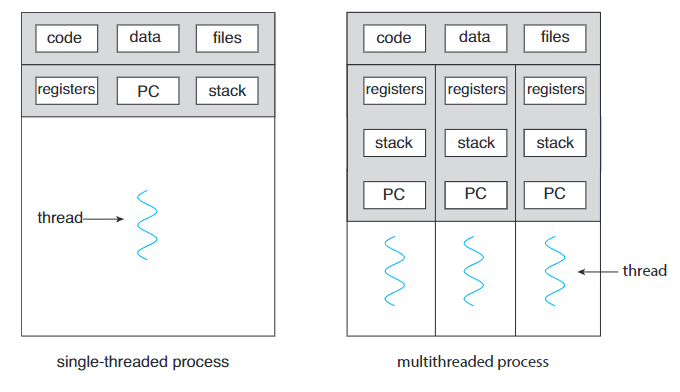
\includegraphics[width=0.309\textwidth]{pic/OS4/Single-threaded and multithreaded processes}
    \caption{Single-threaded and multithreaded processes}
\end{figure}

Benefits:
\begin{itemize}
    \item Responsiveness: interactive applications
    \item Resource Sharing: memory for code and data can be shared.
    \item Economy: creating processes are more expensive.
    \item Utilization of MP Architectures: multi-threading increases concurrency
\end{itemize}

\subsubsection{User Threads}
Thread management done by user-level threads library. 

Three primary thread libraries:
\begin{itemize}
    \item POSIX Pthreads (can also be provided as system library)
    \item Win32 threads
    \item Java threads
\end{itemize}

\subsubsection{Kernel Threads}
Supported by the Kernel. Almost all contemporary OS implements kernel threads.

\subsection{Multithreading Models}
\begin{itemize}\small
    \item Many-to-One: thread mgmt is efficient, but will block if making system call, kernel can schedule only one thread at a time (legacy system(kernel))
    \item One-to-One: more concurrency, but creating thread is expensive
    \item Many-to-Many: flexible    
\end{itemize}

\subsubsection{Many-to-One Model}
Many user-level threads mapped to single kernel thread. 改造老系统, 提供多线程的方式. 
\begin{figure}[!htb]
    \centering
    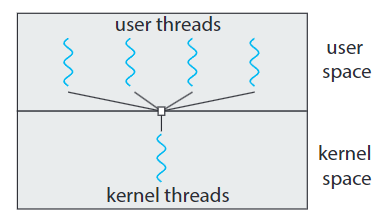
\includegraphics[width=0.309\textwidth]{pic/OS4/Many-to-one model.png}
    \caption{Many-to-one model}
\end{figure}

\subsubsection{One-to-One Model}
Each user-level thread maps to kernel thread

\begin{figure}[!htb]
    \centering
    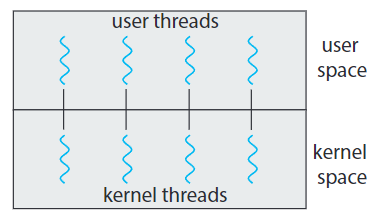
\includegraphics[width=0.309\textwidth]{pic/OS4/One-to-one model.png}
    \caption{One-to-one model}
\end{figure}

\subsubsection{Many-to-Many Model}
Allows many user level threads to be mapped to many kernel threads

Lightweight Process ID 

\begin{figure}[!htb]
    \centering
    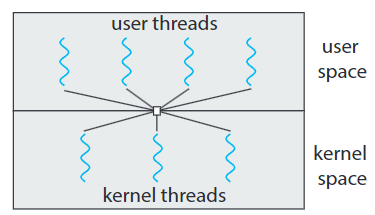
\includegraphics[width=0.309\textwidth]{pic/OS4/Many-to-many model}
    \caption{Many-to-many model}
\end{figure}


\subsubsection{Two-level Model}
Similar to M:M, except that it allows a user thread to be bound to kernel thread

\begin{figure}[!htb]
    \centering
    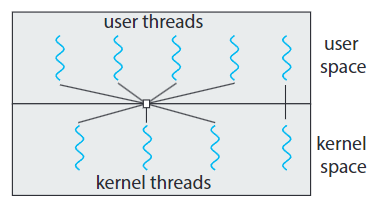
\includegraphics[width=0.309\textwidth]{pic/OS4/Two-level Model}
    \caption{Two-level Model}
\end{figure}


\subsection{Threading Issues}
\subsubsection{Semantics of fork() and exec()}
Does fork() duplicate only the calling thread or all threads? 可以复制全部也可以仅复制本线程. 

exec() will replace the entire process.

\subsubsection{Signal Handling}
signal handler

\subsubsection{Thread Cancellation}
Terminating a thread before it has finished. Two general approaches:
\begin{itemize}
    \item Asynchronous cancellation
    \item Deferred cancellation
\end{itemize}

\subsubsection{Thread Pools}
Create a number of threads in a pool where they await work

\subsubsection{Thread Specific Data}
Thread-Local Storage (TLS). Allows each thread to have its own copy of data

\subsubsection{Scheduler Activations}
调度激活. allows an application to maintain the
correct number of kernel threads